%% icnonla23.tex
%% Copyright 2023 Tom M. Ragonneau
\documentclass[optimization]{common/talk}
\usepackage{makecell}
\usetikzlibrary{patterns}
\addbibresource{\bibfile}

% Performance profiles
\usepackage{xstring}
\newcommand{\drawprofiles}[3]{%
    \def\selectsolvers{#1}%
    \def\selectcsv{figures/#2}%
    \def\selectprofile{#3}%
    \def\selectxlabel{Performance ratios}%
    \def\selectylabel{Performance profiles ($\tau = 10^{-#3}$)}%
    %% profiles.tex
%% Copyright 2023 Tom M. Ragonneau
\begin{tikzpicture}
    \pgfplotstableread[col sep=comma]{\selectcsv}\selectcsvread
    \newcommand{\getxmaxcsv}[1]{%
        \pgfplotstablegetrowsof{\selectcsvread}%
        \pgfmathtruncatemacro{\LastRowNo}{\pgfplotsretval-1}%
        \pgfplotstablesort[sort key={#1}]{\csvsorted}{\selectcsvread}%
        \pgfplotstablegetelem{\LastRowNo}{#1}\of{\csvsorted}%
        \pgfmathsetmacro{\selectxmaxcsv}{\pgfplotsretval}%
    }
    \pgfmathparse{\selectsolvers[0]}
    \let\selectsolver\pgfmathresult\relax
    \getxmaxcsv{x\selectprofile_\selectsolver}
    \begin{axis}[%
        width=185pt,%
        xmode=log,%
        log basis x=2,%
        xmin=1,%
        xmax=\selectxmaxcsv^0.55,%
        ymin=0,%
        ymax=1,%
        minor y tick num=1,%
        yminorticks=true,%
        ytick={0,0.2,...,1},%
        cycle list name=profiles,%
        legend pos=south east,%
        xlabel={\selectxlabel},%
        ylabel={\selectylabel},%
        xticklabel style={/pgf/number format/1000 sep={}},%
        /pgfplots/max space between ticks=30,%
    ]
        \pgfmathparse{dim{\selectsolvers}-1}
        \let\selectlastindex\pgfmathresult\relax
        \foreach \i in {0,1,...,\selectlastindex} {%
            \pgfmathparse{\selectsolvers[\i]}%
            \let\selectsolver\pgfmathresult\relax%
            % \StrSubstitute{\selectsolver}{-}{~}[\selectsolverescaped]%
            \addplot table[%
                x=x\selectprofile_\selectsolver,%
                y=y\selectprofile,%
                col sep=comma,%
            ]{\selectcsvread};%
            % \addlegendentryexpanded{\selectsolverescaped}%
            \addlegendentryexpanded{\selectsolver}%
        }
    \end{axis}
\end{tikzpicture}%
}

\title{COBYQA}
\subtitle{A derivative-free trust-region SQP method for nonlinearly constrained optimization}
\date{ICNONLA 2023, Taiyuan, Shanxi, China, 2023}
\author{\href{https://www.tomragonneau.com}{\textbf{Tom M. Ragonneau}} \and \href{https://www.zhangzk.net}{Zaikun Zhang}}
\institute{
    Department of Applied Mathematics\\
    The Hong Kong Polytechnic University\\
    Hung Hom, Kowloon, Hong Kong, China\\[\baselineskip]
    This work was partially supported by the \href{https://cerg1.ugc.edu.hk/hkpfs/index.html}{Hong Kong PhD Fellowship Scheme}.
}
\hypersetup{
    pdfsubject={ICNONLA 2023},
    pdfkeywords={},
}

\begin{document}

\maketitle

\begin{frame}{Derivative-free optimization (DFO)}
    \begin{itemize}
        \item Minimize a function $\obj$ using \alert{function values} but no derivatives.
        \item $\obj$ can be a \alert{black box} resulting from experiments or simulations.
        \begin{center}
            \medskip
            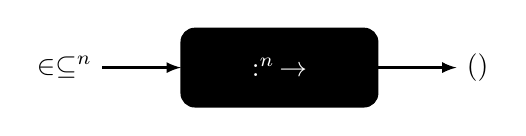
\begin{tikzpicture}
                \draw[-latex,thick] (0,0) node[left] {$\iter \in \fset \subseteq \R^n$} -- (1,0);
                \draw[rounded corners=5pt,fill=black] (1,-.5) rectangle (3.5,.5);
                \node[color=white] at (2.25,0) {$\obj \colon \R^n \to \R$};
                \draw[-latex,thick] (3.5,0) -- (4.5,0) node[right] {$\obj ( \iter )$};
            \end{tikzpicture}
        \end{center}
        \item $\obj$ may be smooth, but $\gradobj$ \alert{cannot} be numerically evaluated.
        \item Evaluations of $\obj$ are \alert{expensive}.
        \item Closely related terms:
        \begin{center}
            \itshape
            blackbox optimization\\
            zeroth-order optimization\\
            simulation-based optimization\\
            gradient-free optimization
        \end{center}
    \end{itemize}
\end{frame}

\begin{frame}{An example of a DFO problem}
    \begin{center}
        \begin{tikzpicture}[scale=.9, every node/.style={transform shape}]
            \uncover<2>{\draw[pattern=north west lines,pattern color=DarkCaramel!40,rounded corners=5pt] (8,3) rectangle (11,4.5);}
            \draw[thick,rounded corners=5pt] (0,0) rectangle (3,1.5);
            \draw[thick,rounded corners=5pt] (0,4) rectangle (3,5.5);
            \draw[thick,rounded corners=5pt] (4,2) rectangle (7,3.5);
            \draw[thick,rounded corners=5pt] (8,1) rectangle (11,2.5);
            \only<1>{\draw[thick,rounded corners=5pt] (8,3) rectangle (11,4.5);}
            \uncover<2>{\draw[thick,rounded corners=5pt,color=DarkCaramel] (8,3) rectangle (11,4.5);}
            \draw[thick,-latex] (3,1) -- (5.5,1) -- (5.5,2);
            \draw[thick] (3,0.5) -- (7.5,0.5) -- (7.5,2.5) -- (7,2.5);
            \draw[thick,-latex] (7.5,1.75) -- (8,1.75);
            \draw[thick] (3,4.75) -- (7.5,4.75) -- (7.5,3) -- (7,3);
            \draw[thick,-latex] (7.5,3.75) -- (8,3.75);
            \node at (0.6,0.75) {
\includegraphics[height=0.75cm]{img/presentation.png}};
            \node at (0.6,4.75) {
\includegraphics[height=0.75cm]{img/checklist.png}};
            \node at (4.6,2.75) {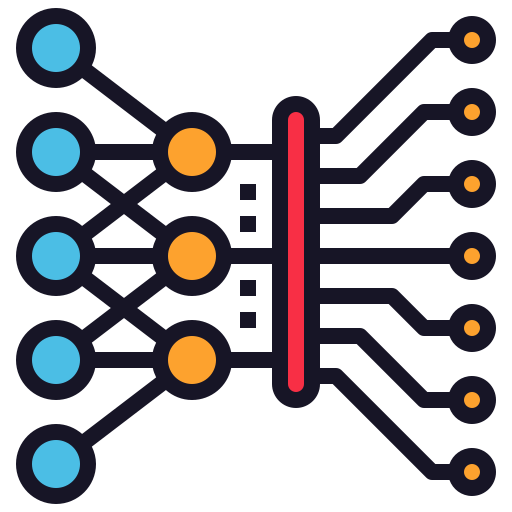
\includegraphics[height=0.75cm]{img/deep-learning.png}};
            \node at (8.6,1.75) {
\includegraphics[height=0.75cm]{img/good.png}};
            \node at (8.6,3.75) {
\includegraphics[height=0.75cm]{img/result.png}};
            \node at (2,0.75) {\makecell{Training\\ data}};
            \node at (2,4.75) {\makecell{Testing\\ data}};
            \node at (6,2.75) {\makecell{Machine\\ learning\\ model}};
            \node at (10,1.75) {\makecell{Training\\ accuracy}};
            \node at (10,3.75) {\makecell{Testing\\ accuracy}};
            \uncover<2>{
                \draw[pattern=north west lines,pattern color=DarkCaramel!40,rounded corners=5pt] (0,2) rectangle (3,3.5);
                \draw[thick,color=DarkCaramel,rounded corners=5pt] (0,2) rectangle (3,3.5);
                \draw[thick,-latex] (3,2.75) -- (4,2.75);
                \node at (0.6,2.75) {
\includegraphics[height=0.75cm]{img/technical-support.png}};
                \node at (2,2.75) {\makecell{Hyper-\\parameters}};
            }
        \end{tikzpicture}

        \pause
        \smallskip

        \begin{block}{Hyperparameter tuning problem}
            \begin{itemize}
                \item How to choose the \alert{hyperparameters}?
                \item \emph{An idea}: optimizing the \alert{testing accuracy}.
                What is the \alert{gradient}?
            \end{itemize}
        \end{block}
    \end{center}
\end{frame}

\begin{frame}{General context}
    We design a method named \alert{COBYQA} for solving
    \begin{equation*}
        \begin{aligned}
            \min_{\iter \in \R^n}   & \quad \obj ( \iter ) \\
            \textrm{s.t.}           & \quad \cub ( \iter ) \le 0, ~ \cancel<2->{\ceq ( \iter ) = 0},\\
                                    & \quad \xl \le \iter \le \xu,
        \end{aligned}
    \end{equation*}
    when derivatives of $\obj$, $\cub$, and $\ceq$ are \alert{unavailable}.

    \pause
    \medskip

    \begin{block}{}
        \begin{itemize}
            \item We omit the equality constraints for simplicity.
            \item COBYQA aims at being a \alert{successor} to COBYLA \parencite{Powell_1994}.
            \item We \alert{implement} COBYQA into a Python solver.
            \item The bound constraints are \alert{unrelaxable}:
            \begin{itemize}
                \item They often represent \alert{inalienable} restrictions.
                \item $\obj$, $\cub$, or $\ceq$ may not be well-defined outside the bounds.
            \end{itemize}
        \end{itemize}
    \end{block}
\end{frame}

\begin{frame}{Table of contents}
    \tableofcontents[hideallsubsections]
\end{frame}

\section{General framework of COBYQA}

\begin{frame}{A derivative-free trust-region SQP method}
    COBYQA iteratively solves the trust-region SQP subproblem
    \begin{align*}
        \min_{\step \in \R^n}   & \quad \transpose{\only<1>{\gradobj}\only<2>{\alert{\gradobjm[k]}} ( \iter[k] )} \step + \frac{1}{2} \transpose{\step} \only<1>{\hesslag[\iter][\iter]}\only<2>{\alert{\hesslagm[k][\iter][\iter]}} ( \iter[k], \lmub[k] ) \step\\
        \textrm{s.t.}           & \quad \only<1>{\cub}\only<2>{\alert{\cubm[k]}} ( \iter[k] ) + \only<1>{\jaccub}\only<2>{\alert{\jaccubm[k]}} ( \iter[k] ) \step \le 0,\\
                                & \quad \xl \le \iter[k] + \step \le \xu,\\
                                & \quad \norm{\step} \le \rad[k],
    \end{align*}
    with $\only<1>{\lag}\only<2>{\alert{\lagm[k]}} ( \iter, \lmub ) = \only<1>{\obj}\only<2>{\alert{\objm[k]}} ( \iter ) + \transpose{\lmub} \only<1>{\cub}\only<2>{\alert{\cubm[k]}} ( \iter )$\only<2>{, given some models $\objm[k]$ and $\cubm[k]$}.

    \pause
    \medskip

    \begin{block}{}
        \begin{itemize}
            \item We only require an approximate solution $\step[k]$.
            \item The solution must satisfy $\xl \le \iter[k] + \step[k] \le \xu$.
            \item The subproblem may be \alert{infeasible}. What is a solution?
        \end{itemize}
    \end{block}
\end{frame}

\begin{frame}{A new Byrd-Omojokun approach}
    We compute $\step[k] = \nstep[k] + \tstep[k]$, where
    \begin{itemize}
        \item the \alert{normal} step $\nstep[k]$ reduces the (possible) constraint violation, and
        \item the \alert{tangential} step $\tstep[k]$ reduces the quadratic objective function.
    \end{itemize}

    \begin{columns}
        \begin{column}{0.4\textwidth}
            \begin{center}
                \begin{tikzpicture}[scale=0.75]
                    % Linear constraints
                    \uncover<1,2,6->{\fill[color=MidnightBlue,opacity=0.4] (-4,-1) -- (-1.5,-1) -- (-0.5,4) -- (-4,4) -- cycle;}
                    \uncover<3-5>{\fill[color=MidnightBlue,opacity=0.4] (-4,-1) -- (-2.1,-1) -- (-1.1,4) -- (-4,4) -- cycle;}
                    \uncover<1,2,6>{\fill[color=MidnightBlue,opacity=0.4] (-4,1) -- (0,4) -- (-4,4) -- cycle;}
                    \uncover<3-5,7->{\fill[color=MidnightBlue,opacity=0.4] (-4,0.125) -- (1,3.875) -- (1,4) -- (-4,4) -- cycle;}

                    % Trust regions
                    \begin{scope}
                        \clip (-4,-1) rectangle (1,4);
                        \draw[fill=DarkCaramel!80,draw opacity=0.7,fill opacity=0.5] (0,0) circle (3);
                        \draw[densely dotted,fill=DarkCaramel!80,opacity=0.7] (0,0) circle (2.5);
                    \end{scope}

                    % Feasible region for the tangential subproblem
                    \begin{scope}
                        \clip (-4,0.125) -- (-1.5,2) -- (-1.1,4) -- (-4,4) -- cycle;
                        \uncover<4-5>{\fill[pattern=north west lines,pattern color=VeniceBlue!70!black,opacity=0.75] (0,0) circle (3);}
                    \end{scope}
                    \begin{scope}
                        \clip (-4,0.125) -- (-27/34,43/17) -- (-0.5,4) -- (-4,4) -- cycle;
                        \uncover<8->{\fill[pattern=north west lines,pattern color=VeniceBlue!70!black,opacity=0.75] (0,0) circle (3);}
                    \end{scope}

                    % Frame and annotations
                    \uncover<5>{
                        \draw[-stealth,thick,VeniceBlue!90!black] (-1.5,2) -- (-2.2,1.7) node[midway,below right] {$\tstep[k]$};
                    }
                    \uncover<9>{
                        \draw[-stealth,thick,VeniceBlue!90!black] (-1.5,2) -- (-0.9,2.7) node[midway,below right] {$\tstep[k]$};
                    }
                    \uncover<2->{\draw[-stealth,thick,RawSienna] (0,0) -- (-1.5,2) node[midway,above right] {$\nstep[k]$};}
                    \draw[fill] (0,0) circle (1.4pt) node[below right] {$\iter[k]$};
                    \draw[thick] (-4,-1) rectangle (1,4);
                \end{tikzpicture}
            \end{center}
        \end{column}
        \begin{column}{0.6\textwidth}
            \begin{tikzpicture}
                \draw[fill=DarkCaramel!80,draw opacity=0.7,fill opacity=0.5] (0,0) circle (.2);
                \node[right] at (.4,0) {Trust region};
                \draw[densely dotted,fill=DarkCaramel!80,opacity=0.7] (0,-0.6) circle (.2);
                \node[right] at (.4,-0.6) {Reduced trust region};
                \fill[color=MidnightBlue,opacity=0.4] (-.2,-1.4) rectangle (.2,-1);
                \node[right] at (.4,-1.2) {Linear constraints};
                \uncover<4->{
                    \fill[pattern=north west lines,pattern color=VeniceBlue!70!black,opacity=0.75] (-.2,-2) rectangle (.2,-1.6);
                    \node[right] at (.4,-1.8) {Feasible region for $\tstep[k]$};
                }
            \end{tikzpicture}

            \bigskip

            \alert<1-5>{Standard} approach\footnotemark\ vs.\ \alert<6->{new} one.
        \end{column}
    \end{columns}

    \uncover<9>{The feasible region for $\tstep[k]$ is \alert{wider} in the new approach.}
    \footnotetext{See \textcite[\S 15.4.4]{Conn_Gould_Toint_2000}.}
\end{frame}

\begin{frame}{A new Byrd-Omojokun approach (cont'd)}
    \alert{\only<1>{Standard}\only<2>{New}} approach:
    \begin{itemize}
        \item The normal step $\nstep[k]$ solves approximately (for some $\zeta < 1$)
        \begin{align*}
            \min_{\step \in \R^n}   & \quad \norm[\big]{\big[ \cubm[k] ( \iter[k] ) + \jaccubm[k] ( \iter[k] ) \step \big]^+}\\
            \textrm{s.t.}           & \quad \xl \le \iter[k] + \step \le \xu,\\
                                    & \quad \norm{\step} \le \zeta \rad[k].
        \end{align*}
        \item The tangential step $\tstep[k]$ solves approximately
        \begin{align*}
            \min_{\step \in \R^n}   & \quad \transpose{\big[ \gradobjm[k] ( \iter[k] ) + \hesslagm[k][\iter][\iter] ( \iter[k], \lmub[k] ) \nstep[k] \big]} \step + \frac{1}{2} \transpose{\step} \hesslagm[k][\iter][\iter] ( \iter[k], \lmub[k] ) \step\\
            \textrm{s.t.}           & \quad \jaccubm[k] ( \iter[k] ) \step \le \alert{\only<1>{0}\only<2>{[\cubm[k](\iter[k]) + \jaccubm[k] ( \iter[k] ) \nstep[k]]^-}},\\
                                    & \quad \xl \le \iter[k] + \nstep[k] + \step \le \xu,\\
                                    & \quad \norm{\nstep[k] + \step} \le \rad[k].
        \end{align*}
    \end{itemize}
\end{frame}

\section{Interpolation-based models}

\begin{frame}{Interpolation-based quadratic models}
    COBYQA builds \alert{quadratic} models of $\obj$ and $\cub$ by interpolation.

    \begin{block}{Derivative-free symmetric Broyden update \parencite{Powell_2004}}
        The $k$th model $\objm[k]$ of $\obj$ solves
        \begin{align*}
            \min_{Q \in \mathcal{Q}_n}  & \quad \norm[\big][fro]{\nabla^2 \objm[k - 1] - \nabla^2 Q}\\
            \textrm{s.t.}               & \quad Q(y) = \obj(y), ~ y \in \xpt[k],
        \end{align*}
        for some interpolation set $\xpt[k] \subseteq \R^n$ (similar for $\cubm[k]$).
    \end{block}

    \begin{itemize}
        \item We \alert{recycle} $\xpt[k + 1] = ( \xpt[k] \cup \set{\iter[k] + \step[k]} ) \setminus {\bar{y}}$ for some bad point $\bar{y} \in \xpt[k]$.
        \item To compute $\objm[k]$, we only need to solve a \alert{linear} system.
    \end{itemize}

    \underline{Some alternatives}: \textcite{Conn_Scheinberg_Toint_1997a,Conn_Scheinberg_Toint_1997b,Conn_Scheinberg_Toint_1998,Wild_2008,Custodio_Rocha_Vicente_2010,Bandeira_Scheinberg_Vicente_2012,Zhang_2014,Xie_Yuan_2023}.
\end{frame}

\section{Many difficulties arise}

\begin{frame}{A lot of questions must be addressed}
    \begin{itemize}
        \item How to calculate the steps $\nstep[k]$ and $\tstep[k]$ numerically?\\
        \textcolor{FernGreen}{COBYQA adapts the truncated conjugate gradient method.}
        \item What is the approximate Lagrange multiplier $\lmub[k]$?\\
        \textcolor{FernGreen}{We choose the least-squares Lagrange multiplier.}
        \item Which merit function should we use?\\
        \textcolor{FernGreen}{COBYQA uses the $\ell_2$-merit function.}
        \item How to update the penalty parameter?\\
        \textcolor{FernGreen}{The update incorporates}
        \begin{itemize}
            \item \textcolor{FernGreen}{a theoretical value for the exactness of the merit function, and}
            \item \textcolor{FernGreen}{a strategy used by Powell in COBYLA.}
        \end{itemize}
    \end{itemize}

    \medskip

    These questions (and many more) are addressed in \textcite{Ragonneau_2022}.
\end{frame}

\begin{frame}{A crucial difficulty in the implementation}
    \begin{itemize}
        \item What if the interpolation set $\xpt[k]$ is almost nonpoised?\\
        \textcolor{FernGreen}{A well-known approach: a geometry-improving mechanism.\footnote{See \textcite{Conn_Scheinberg_Vicente_2008a,Conn_Scheinberg_Vicente_2008b,Fasano_Morales_Nocedal_2009}.}}
    \end{itemize}

    \medskip

    \begin{block}{This is a central difficulty in the implementation of DFO methods}
        \begin{center}
            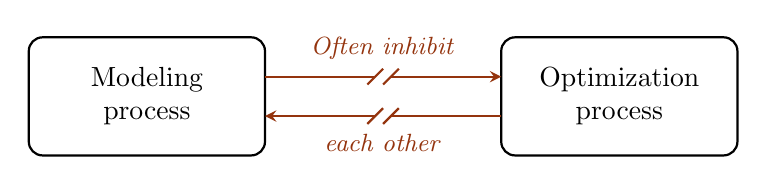
\begin{tikzpicture}
                \draw[rounded corners=5pt,thick] (0,0) rectangle (3,1.5);
                \draw[rounded corners=5pt,thick] (6,0) rectangle (9,1.5);
                \draw[thick,RawSienna] (3,1) -- (4.4,1);
                \draw[-stealth,thick,RawSienna] (4.6,1) -- (6,1);
                \draw[thick,RawSienna] (4.3,0.9) -- (4.5,1.1);
                \draw[thick,RawSienna] (4.5,0.9) -- (4.7,1.1);
                \draw[thick,RawSienna] (6,0.5) -- (4.6,0.5);
                \draw[-stealth,thick,RawSienna] (4.4,0.5) -- (3,0.5);
                \draw[thick,RawSienna] (4.3,0.4) -- (4.5,0.6);
                \draw[thick,RawSienna] (4.5,0.4) -- (4.7,0.6);
                \node at (1.5,0.75) {\makecell{Modeling\\ process}};
                \node at (7.5,0.75) {\makecell{Optimization\\ process}};
                \node[above,text=RawSienna] at (4.5,1.1) {\small\emph{Often inhibit}};
                \node[below,text=RawSienna] at (4.5,0.4) {\small\emph{each other}};
            \end{tikzpicture}
        \end{center}

        \begin{itemize}
            \item The iterates $\set{x^k}$ likely lie on a particular path.
            \item The modeling process does \alert{not} ponder the optimization problem.
        \end{itemize}
    \end{block}
\end{frame}

\begin{frame}{Management of the trust-region radius}
    \begin{block}{We maintain $\rad[k]$ and a lower bound $\radlb[k] \le \rad[k]$}
        \begin{itemize}
            \item The lower bound $\radlb[k]$ is \alert{never} increased.
            \item We update $\rad[k]$ in the usual way, but we \alert{always} have $\rad[k] \ge \radlb[k]$.
            \item This strategy is adapted from \alert{Powell}'s methods (e.g., NEWUOA).
        \end{itemize}
    \end{block}

    The value of $\radlb[k]$ is an indicator of the current \alert{resolution}.

    \begin{itemize}
        \item Without $\rad[k] \ge \radlb[k]$, the value of $\rad[k]$ may become too small.
        \item It prevents the interpolation points from \alert{concentrating} too much.
        \item The value of $\radlb[k]$ is only \alert{decreased} when necessary.
        \item Hence, stopping when $\radlb[k] \le \radlb[\textrm{end}]$ is \alert{reasonable} ($\radlb[\textrm{end}] > 0$).
    \end{itemize}
\end{frame}

\section{Implementation and experiments}

\begin{frame}[fragile]{The Python implementation of COBYQA}
    \begin{block}{From \textcite{Powell_2006}}
        \begin{quoting}
            \small%
            The development of NEWUOA has taken nearly \alert{three years}.
            The work was very \alert{frustrating} [\dots]
        \end{quoting}
        The development of COBYQA was \alert{not easier}.
    \end{block}

    We implemented COBYQA in \alert{Python} and made it publicly available.

    \begin{center}
        \qrcode{https://www.cobyqa.com}\\[1ex]
        \href{https://www.cobyqa.com}{\texttt{www.cobyqa.com}}
    \end{center}

    \begin{block}{}
        \texttt{\$ pip install cobyqa}
    \end{block}

    % \underline{Installation}: \texttt{pip install cobyqa}

    % \begin{columns}
    %     \begin{column}{0.4\textwidth}
    %         \begin{center}
    %             \qrcode{https://www.cobyqa.com}\\[1ex]
    %             \href{https://www.cobyqa.com}{\texttt{www.cobyqa.com}}
    %         \end{center}
    %     \end{column}
    %     \begin{column}{0.6\textwidth}
    %     \end{column}
    % \end{columns}
\end{frame}

\begin{frame}{Comparing COBYQA with existing DFO solvers}
    \begin{itemize}
        \item We assess the quality of points based on the merit function
        \begin{equation*}
            \varphi(\iter) =
            \begin{cases}
                \obj(\iter)                           & \text{if $v_{\infty}(x) \le 10^{-10}$,}\\
                \infty                                & \text{if $v_{\infty}(x) \ge 10^{-5}$,}\\
                \obj(\iter) + 10^5 v_{\infty}(\iter)  & \text{otherwise,}
            \end{cases}
        \end{equation*}
        where $v_{\infty}$ denotes the $\ell_{\infty}$-constraint violation.
        \item The problems are from the \alert{CUTEst} set.
        \item The problems are of \alert{dimension} at most \num{50} (this is \alert{not} small).
        \item Problems with \alert{unrelaxable} bounds replace $\obj$ with
        \begin{equation*}
            \tilde{\obj}(x) =
            \begin{cases}
                \obj(x) & \text{if $\xl \le x \le \xu$,}\\
                \infty  & \text{otherwise.}
            \end{cases}
        \end{equation*}
    \end{itemize}
\end{frame}

\begin{frame}{Performance of the new Byrd-Omojokun approach}
    We compare the new and the standard Byrd-Omojokun approaches
    \begin{itemize}
        \item on \alert{linearly} and \alert{nonlinearly constrained} problems,
        \item in the implementation of COBYQA.
    \end{itemize}

    \smallskip

    \begin{center}
        \drawprofiles{{"New","Standard"}}{plain-1-50-perf-byrd-omojokun-nlqo.csv}{4}
    \end{center}
\end{frame}

\begin{frame}{Performance on linearly constrained problems}
    We compare COBYQA, LINCOA, and COBYLA
    \begin{itemize}[<+->]
        \item on \alert{linearly constrained} problems,
        \item with \alert{inviolable} bounds.
    \end{itemize}

    \smallskip

    \begin{center}
        \only<1>{\drawprofiles{{"COBYQA","LINCOA","COBYLA"}}{plain-1-50-perf-cobyla-cobyqa-lincoa-nl.csv}{4}}%
        \only<2>{\drawprofiles{{"COBYQA","LINCOA","COBYLA"}}{plain-1-50-perf-cobyla-cobyqa-lincoa-nl-bounds.csv}{4}}
    \end{center}
\end{frame}

\begin{frame}{Performance on nonlinearly constrained problems}
    We compare COBYQA and COBYLA
    \begin{itemize}[<+->]
        \item on \alert{nonlinearly constrained} problems,
        \item with \alert{inviolable} bounds.
    \end{itemize}

    \smallskip

    \begin{center}
        \only<1>{\drawprofiles{{"COBYQA","COBYLA"}}{plain-1-50-perf-cobyla-cobyqa-qo.csv}{4}}%
        \only<2>{\drawprofiles{{"COBYQA","COBYLA"}}{plain-1-50-perf-cobyla-cobyqa-qo-bounds.csv}{4}}
    \end{center}
\end{frame}

\begin{frame}{Comparison with COBYLA}
    We compare COBYQA and COBYLA on \alert{all} 388 problems.

    \bigskip

    \begin{center}
        \drawprofiles{{"COBYQA","COBYLA"}}{plain-1-50-perf-cobyla-cobyqa-ubnlqo.csv}{4}
    \end{center}
\end{frame}

\section{Conclusion}

\begin{frame}{Conclusion}

    \begin{itemize}
        \item COBYQA already received \alert{positive} feedback from practitioners.
        \item It will soon be included in
        \begin{itemize}
            \item \href{https://www.pdfo.net}{PDFO} as a successor for COBYLA, and
            \item \href{https://gemseo.readthedocs.io}{GEMSEO}, an \alert{industrial} software package for MDO.
        \end{itemize}
        \item We will soon investigate the convergence properties of COBYQA.
    \end{itemize}

    For more information, visit:

    \medskip

    \begin{columns}
        \begin{column}{\textwidth/3}
            \begin{center}
                \qrcode{https://www.cobyqa.com}\\[1ex]
                \href{https://www.cobyqa.com}{COBYQA}
            \end{center}
        \end{column}
        \begin{column}{\textwidth/3}
            \begin{center}
                \qrcode{https://www.tomragonneau.com}\\[1ex]
                \href{https://www.tomragonneau.com}{My website}
            \end{center}
        \end{column}
        \begin{column}{\textwidth/3}
            \begin{center}
                \qrcode{https://tomragonneau.com/documents/thesis.pdf}\\[1ex]
                \href{https://tomragonneau.com/documents/thesis.pdf}{My thesis}
            \end{center}
        \end{column}
    \end{columns}
\end{frame}

\appendix

\begin{frame}[t,allowframebreaks]{References}
    \printbibliography[heading=none]
\end{frame}

\end{document}
